%
%  $Author: ienne $
%  $Date: 1995/09/15 15:20:59 $
%  $Revision: 1.4 $
%

% \documentclass[10pt,journal,cspaper,compsoc]{IEEEtran}   %%%tc version
\documentclass[10pt, conference]{IEEEtran}
%\documentclass[conference,compsoc]{IEEEtran}
%\documentclass[10pt, conference]{IEEEtran}
%\documentclass[times, 10pt,onecolumn]{article}
\usepackage{amsmath, amssymb, enumerate}

%%%%%%%%%%%%%%%% page control%%%%%%%%%%%%%%%%%
%\usepackage[margin=0.75in]{geometry}

%\linespread{0.991}  %%%%%%%%%%%%%%%%%%%%%%%%%%%%%%%%% this is really useful
%\usepackage{cite}
\usepackage{fancybox}
\usepackage{amsfonts}
%\usepackage{algorithm}
%\usepackage[noend]{algorithmic}
\usepackage[usenames]{color}
%\usepackage{colortbl}
%\usepackage[ figure, boxed, vlined]{algorithm2e}
%\usepackage[linesnumbered,vlined]{algorithm2e}
%\usepackage[lined,boxed]{algorithm2e}
\usepackage{listings}

\usepackage[linesnumbered,vlined]{algorithm2e}
\usepackage{graphicx}
\usepackage{times}
\usepackage{psfrag}
\usepackage{subfigure}
\usepackage{caption}
%\usepackage{subcaption}
\usepackage{multirow}
%\usepackage{setspace}
%\usepackage{listings}
\usepackage{epsfig}
%\usepackage{epstopdf}
%\usepackage[font=small,labelfont=bf]{caption}
\usepackage{url}

\usepackage{color}
\def\fixme#1{\typeout{FIXED in page \thepage : {#1}}
%\bgroup \color{red}{} \egroup}
\bgroup \color{red}{[FIXME: {#1}]} \egroup}


\usepackage[pdftex]{hyperref}
\usepackage{rotating,tabularx}

\interfootnotelinepenalty=10000

%% Define a new 'leo' style for the package that will use a smaller font.
\makeatletter
\def\url@leostyle{%
  \@ifundefined{selectfont}{\def\UrlFont{\sf}}{\def\UrlFont{\small\ttfamily}}}
\makeatother

%\documentstyle[times,art10,twocolumn,latex8]{article}

%-------------------------------------------------------------------------
% take the % away on next line to produce the final camera-ready version
\pagestyle{plain}
%\thispagestyle{empty}
%\pagestyle{empty}

\newtheorem{theorem}{Theorem}
\newtheorem{lemma}[theorem]{Lemma}

%% remaining budget share, used in task stall section.
\newcommand{\bottomrule}{\hline}
\newcommand{\toprule}{\hline}
\newcommand{\midrule}{\hline}
%-------------------------------------------------------------------------
\begin{document}

\title{DeepPicar:​ ​A​ ​Low-cost​ ​Deep​ ​Neural​ ​Network-based​ ​Autonomous​ ​Car}
\author{Michael Garrett Bechtel, Elise McEllhiney, Heechul Yun\\
\{m783b224, e908m429, heechul.yun\}@ku.edu\\
University of Kansas, USA\\ 
}

\maketitle
\thispagestyle{empty}
\begin{abstract}
In order to effectively research autonomous vehicles, a real-time
capable platform is required. Such platforms can be hard to obtain, or
build, as the necessary components can be expensive. In this paper,
we present a low-cost alternative platform that utilizes a Raspberry
Pi 3 Model B, along with a single external camera sensor, to perform
all necessary self-driving operations. A convolutional neural network
(CNN) is employed and trained with input from a human driver to
navigate a custom made track. We display the real-time efficacy of our
platform in experiments with varying amounts of computational resources
and/or intensive AI workloads. To gain a better understanding of our
platform's potential, we compare it to other embedded computing
platforms to determine which are suitable for autonomous driving
research.
\end{abstract}

%-------------------------------------------------------------------------
\section{Introduction} \label{sec:intro}

% broad context:
% - advance in ai sparked interests in the robotics application, such as
%   self-driving cars.
% - in particular, deep neural network models are increasingly used
%   for perception and control of a vehicle. say. AI workloads.
%
%
Autonomous cars have been a topic of increasing interest in recent
years as many companies are actively developing related hardware
and software technologies toward fully autonomous driving capability without
any human intervention. Deep neural networks (DNNs) have been
sucessfully applied in various perception and control tasks in 
recent years, and they are important workloads for autonomous vehicles
as well. For example, Tesla Model S was known to use a specialized
chip (MobileEye EyeQ), which uses a deep neural network for vision-based
real-time obstacle detection and avoidance. More recently, researchers
are investigating DNN based end-to-end control of
cars~\cite{Bojarski2016} and other robots. It is expected that more
DNN based Artifical Intelligence workloads may be used in future
autonomous vehicles.

% big problem
Executing these AI workloads on a embedded computing platform that can
be used in a car poses several additional challenges. First, many AI
workloads in vehicles are computationaly demanding and have strict
real-time requirements. For example, latency in a vision-based object
detection task may directly linked to safety of the vehicle. This
requires a high computing capacity as well as means to guaranteeing
the timings. On the other hand, the computing hardware platform must
also satisfy cost, size, weight, and power constraints, which require
highly efficient computing platform. These two conflicting
requirements  complicate the platform selection process as observed in
~\cite{Otterness2017}, which evaluated vision workloads on
NVIDIA's Tegra TX1 platform.
%% For example, while today's self-driving car
%% prototype equip more \$100,000 
%% of computers and sensors~\cite{juliussen2014emerging}, a study
%% found that aveage consumers are willing to pay much less amount of
%% extra cost for a self-driving capability~\cite{Daziano2017}.
%% https://qz.com/924212/what-it-really-costs-to-turn-a-car-into-a-self-driving-vehicle/ 

% related work and remaing problems
To understand what kind of computing hardware is needed for AI
workloads, we need a testbed and realistic workloads. While a real car
testbed would be most ideal, it is not only highly expensive but also
poses serious safety concerns that hinder development and exploration.
Therefore, there is a strong need for safer and less costly testbeds
that still employ state-of-the-art AI technologies. There are already
several relatively inexpensive RC-car based testbeds, such as MIT
RaceCar~\cite{shin2017project} and UPenn's F1$/$10 racecar~\cite{upennf1tenth}.
However, these RC-car testbeds still cost more than \$3,000.

% our goals
Instead, we want to build a low cost testbed that still employs the
state-of-the art AI technologies. Specifically, we focus on a deep
convolutional neural network (CNN) based end-to-end control system,
which was developed for a real self-driving car, NVIDIA
DAVE-2~\cite{Bojarski2016}, and use the same moethodology on a
smaller, safer and less costly setup. In developing the testbed, our
goals are (1) to analyze real-time issues in DNN based end-to-end
control; (2) to evalute real-time performance of contemporarly embedded
multicore platforms for the AI workloads.

% DeepPicar introduction
In this paper, we present DeepPicar, a low-cost autonomous car
platform for research and education. From hardware perspective, 
DeepPicar is comprised of a Raspberry Pi 3 Model B quad-core
computer, a web camera and a RC car, all of which are affordable
components (less than \$100 in total).
The DeepPicar, however, employs state-of-the-art AI
techonologies, including a vision-based end-to-end control system that
utilizes a deep convolutional nueral network (CNN).
The network receives an image frame from a single forward
looking camera as input and generates a predicted steering angle
value as output at each control period in \emph{real-time}. 
The network has 9 layers, about 27 million connections
and 250 thousand parameters (weights).
The network architecture is identifical to that of NVIDIA's DAVE-2
self-driving car~\cite{Bojarski2016}, which uses much more powerful
computer (Drive PX computer~\cite{drivepx}) than Raspberry Pi~3.
We chose to use Pi 3 not only because of its
affordability but also because it is representative
of today's mainstream low-end embedded multicore platforms, found in
smartphones and other embedded devices.

%% Other than the difference in scale (RC car vs. real car), the only other
%% differences between the two systems---from the computing
%% perspective---are that our system is implemented in
%% TensorFlow~\cite{abadi2016tensorflow} and runs on a Raspberry Pi 3
%% whereas NVIDIA's DAVE-2 systems is implemented in Torch
%% 7~\cite{collobert2011torch7} and runs on a Drive PX computer (NVIDIA's
%% automotive specialized computing system~\cite{drivepx}), which is more
%% powerful but also more expensive.

% how we trained (maybe moved to a later section)
We apply a standard imitation learning methodology to train the cat to
follow tracks on the ground. We collect data for 
taining and validation by manually  
controlling the RC car and recording the vision (from the webcam
mounted on the RC-car) and the human control inputs. We then train the
network offline using the collected data on a desktop computer, which
equips a NVIDIA GTX 1060 GPU. Finally, the trained network is copied
back to the Raspberry Pi, which is then used to perform interference
operations---locally on the Pi---in the car's main control loop in
real-time. For real-time control, each inference operation must
be completed within the desired control period. (e.g., 50ms period for
20Hz control frequency.)
% how we evaluated (in terms real-time performance)

% what are our findings?
\fixme{TBD: Summary of our findings}

% contributions
The {\bf contributions} of this paper are as follows:
\begin{itemize}
  \item We present the design and implementation of a
    low-cost autonomous vehicle testbed DeepPicar, which utilizes the
    state-of-the-art aritificial intelligence techniques.
  \item We provide an analysis and case-study of real-time issues in the
    DeepPicar.
  \item We systematically compare real-time computing capabilities of
    multiple embedded computing platforms in the contex of a
    vision-based autnomous driving.
\end{itemize}

%% The DeepPicar is comprised of a Raspberry
%% Pi 3 Model B, a camera and a low cost RC car.

%% By creating and using the Picar platform, we seek to accomplish the 
%% following three goals. First, the significant reduction of the overall
%% cost required 
%% would make autonomous driving research more accessible to interested
%% individuals/parties. Furthermore, it would remove the concerns of
%% creating replacement platforms as each part, or the entire system,
%% could be replaced relatively inexpensively. Second, the utilization of
%% a more cost-efficient platform would allow for a better understanding
%% of the performance requirements necessary for efficiently operating
%% autonomous vehicles. Finally, we strive to achieve the ability to
%% compare the real-time performance of multiple embedded computing
%% platforms. 

%% We display the efficacy of the Picar by training and testing the
%% DeepTesla DNN \cite{} in a custom-made environment. We find that the
%% Picar is capable of consistently accomplishing all real-time
%% operations required for autonomous driving in a 50 millisecond frame. 

The remaining sections of the paper are as follows: Section II gives
an overview of the platform, including the high-level system and the
methods used for training and inference. Section III discusses the
ways/methodologies in which training data was collected. Section IV
outlines the network architecture. This is followed by the real-time
DNN inferencing in Section V. Section VI reviews the online/offline
training done with the platform, with an evaluation given in Section
VII. Section VIII gives a discussion of related works, and the paper
finishes with conclusions in Section IX. 


%% it is necessary that all real-time operations are successfully
%% performed prior to their deadlines. This requires that the AV platform
%% be capable of completing all necessary computations in a timely
%% manner, while maintaining a high level of accuracy. Consequently, the
%% cost of creating a platform capable of self-driving can be relatively
%% high, especially in the current cost-sensitive climate of the
%% automotive industry \cite{}. The overall price for an autonomous
%% vehicle platform currently acts as a bottleneck, especially from an
%% academic standpoint, where cost is an important factor. For many
%% researchers and students, the charge associated with autonomous
%% vehicle research is a significant barrier. These same parties may also
%% be deterred from participating in autonomous vehicle research due to
%% the potential for their developed platforms to break in the
%% experimental process. The idea of building one relatively expensive
%% platform may not be too daunting for some, but the notion of
%% potentially making multiple identical platforms in case of accidents
%% may be overwhelming.
%% Toward this end, we explore the possibility of
%% developing a low-cost system that still employs state-of-the-art AI
%% technologies and is capable of executing real-time autonomous vehicle
%% operations. 


\section{Background and Related Work} \label{sec:background}

In this section, we provide background and related work on the
application of deep learning in robotics, particularly autonomous
vehicles. 

\subsection{End-to-End Deep Learning for Autonomous Vehicles}

%% - explosion of AI
%% - in particular, application of DNN in perception and control of robotics systems.
%% - end-to-end control is a promising technique.
%%   levine's publications?
%% - examples: nvidia's DAVE-II prototype, forest navigating drone
%% challenge problem: computing at low cost?

To solve the problem of autonomous driving, a standard approach has
been decomposing the problem into multiple sub-problems,
such as lane marking detection, path planning, and low-level
control, which together form a processing pipeline~\cite{Bojarski2016}.
Recently, researchers are exploring another approach that dramatically
simplifies the standard control pipeline by applying deep neural
networks to directly produce control outputs from senor
inputs~\cite{Levine2016}. Figure~\ref{fig:end-to-end-control}
shows the differences between the two approaches.

\begin{figure}[h]
  \centering
  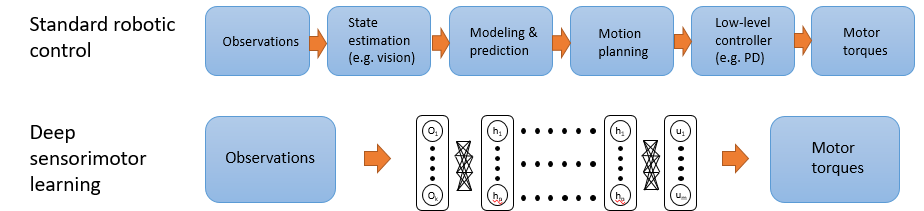
\includegraphics[width=.75\textwidth]{figs/endtoend_redrawn}
  \caption{Standard robotics control vs. DNN based end-to-end
    control. Adopted from ~\cite{Levine2017cs294}.}
  \label{fig:end-to-end-control}
\end{figure}

The use of neural networks for end-to-end control of autonomous
car was first demonstrated in late 1980s~\cite{Pomerleau1989},
using a small 3-layer fully connected neural network; and subsequently
in a DARPA Autonomous Vehicle (DAVE) project in early
2000s~\cite{LeCun:04}, using a 6 layer convolutional neural network
(CNN); and most recently in NVIDIA's DAVE-2
project~\cite{Bojarski2016}, using a 9 layer CNN. In all of these projects,
the neural network models take raw image pixels as input and directly
produce steering control commands, bypassing all intermediary steps and
hand-written rules used in the conventional robotics control approach.  
NVIDIA's latest effort reports that their trained CNN
autonomously controls their modified cars on public roads without human
intervention~\cite{Bojarski2016}.

Using deep neural networks involves two distinct
phases~\cite{NVIDIA2015}. The first
phase is \emph{training} during which the weights of the network are
incrementally updated by backpropagating errors it sees from the
training examples. Once the network is trained---i.e., the weights of
the network minimize errors in the training examples---the next phase
is \emph{inferencing}, during which unseen data is fed to the network
as input to produce predicted output (e.g., predicted image
classification). In general, the training phase is more computationally
intensive and requires high throughput, which is generally not
available on embedded platforms. The inferencing phase, on the
other hand, is relatively less computationally intensive and latency becomes
as important, if not moreso, as computational throughput, because many
use-cases have strict real-time requirements (e.g., search query
latency).

%% \cite{Levine2016}: ``In this paper, we aim to answer
%% the following question: does training the perception and control
%% systems jointly end-toend 
%% provide better performance than training each component separately?''

%% \cite{Bojarski2016} nvidia paper
%% ``We trained a convolutional neural network (CNN) to map raw pixels from
%% a sin- gle front-facing camera directly to steering commands.''

%% ``Compared to explicit decomposition of the problem, such as lane
%% marking detec- tion, path planning, and control, our end-to-end system
%% optimizes all processing steps simultaneously. We''

%% UPenn's f1/10 BOM: $3,628.37
%% http://f1tenth.org/
%% http://selfdrivingcars.mit.edu/
%% http://fast.scripts.mit.edu/racecar/
%% https://github.com/mit-racecar
%% https://mit-racecar.github.io/

\subsection{Embedded Computing Platforms for Real-Time Inferencing}
Real-time embedded systems, such as an autonomous vehicle, present
unique challenges for deep learning, as the computing platforms of such
systems must satisfy two often conflicting goals~\cite{Otterness2017}:
%% Recent successes in AI, including NVIDIA's DAVE-2 showing, are due
%% in large part to the increased computing performance,
%% which afforded researchers to train and use ever deeper neural networks with
%% high accuracy.
%% For practical applications, the computer platform in an
%% autonomous vehicle must satisfy two often conflicting goals:
The platform must provide 
enough computing capacity for real-time processing of computationally
expensive AI workloads (deep neural networks);
The platform must also satisfy various
constraints such as cost, size, weight, and power consumption limits.

Accelerating AI workloads, especially inferencing
operations, has received a lot of attention from academia and industry
in recent years as applications of deep learning are broadening to
areas of real-time embedded systems such as autonomous vehicles. These
efforts include the development of various heterogeneous architecture-based 
system-on-a-chips (SOCs) that may include multiple cores, GPU,
DSP, FPGA, and neural network optimized ASIC hardware~\cite{Jouppi2017}.
Consolidating multiple tasks on SoCs with lots of shared hardware
resources while guaranteeing real-time performance is also an active
research area, which is orthogonal to improving raw
performance. Consolidation is necessary for efficiency, but unmanaged 
interference can nullify the benefits of consolidation~\cite{Kim2016}.
For these reasons, finding a good computing platform is a
non-trivial task, one that requires a deep understanding of the
workloads and the hardware platform being utilized.

The primary objectives of this study are to understand (1) the
necessary computing performance for applying AI technology-based
robotics systems, and (2) what kind of computing architecture and
runtime supports are most appropriate for such workload. To
achieve these goals, we implement a low-cost autonomous car platform
as a case-study and systematically conduct experiments, which we will 
describe in the subsequent sections.


\section{DeepPicar Overview}\label{sec:overview}

In this section, we provide an overview of our DeepPicar platform.
In developing DeepPicar, one of our primary goals is to faithfully
replicate NVIDIA's DAVE-2 system on a smaller scale using a low cost
multicore platform, the Raspberry Pi 3. Because Raspberry Pi 3's
computing performance is much lower than that of the DRIVE
PX~\cite{drivepx} platform used in DAVE-2, we are interested in if,
and how, we can process 
computationally expensive neural network operations in
real-time. Specifically, inferencing (forward pass processing)
operations must be completed within each control period
duration---e.g., a WCET of 33.3 ms for 30Hz control 
frequency---locally on the Pi 3 platform, although training of the 
network (back-propagation for weight updates) can be done offline and 
remotely using a desktop computer.

\begin{figure}[h]
  \centering
  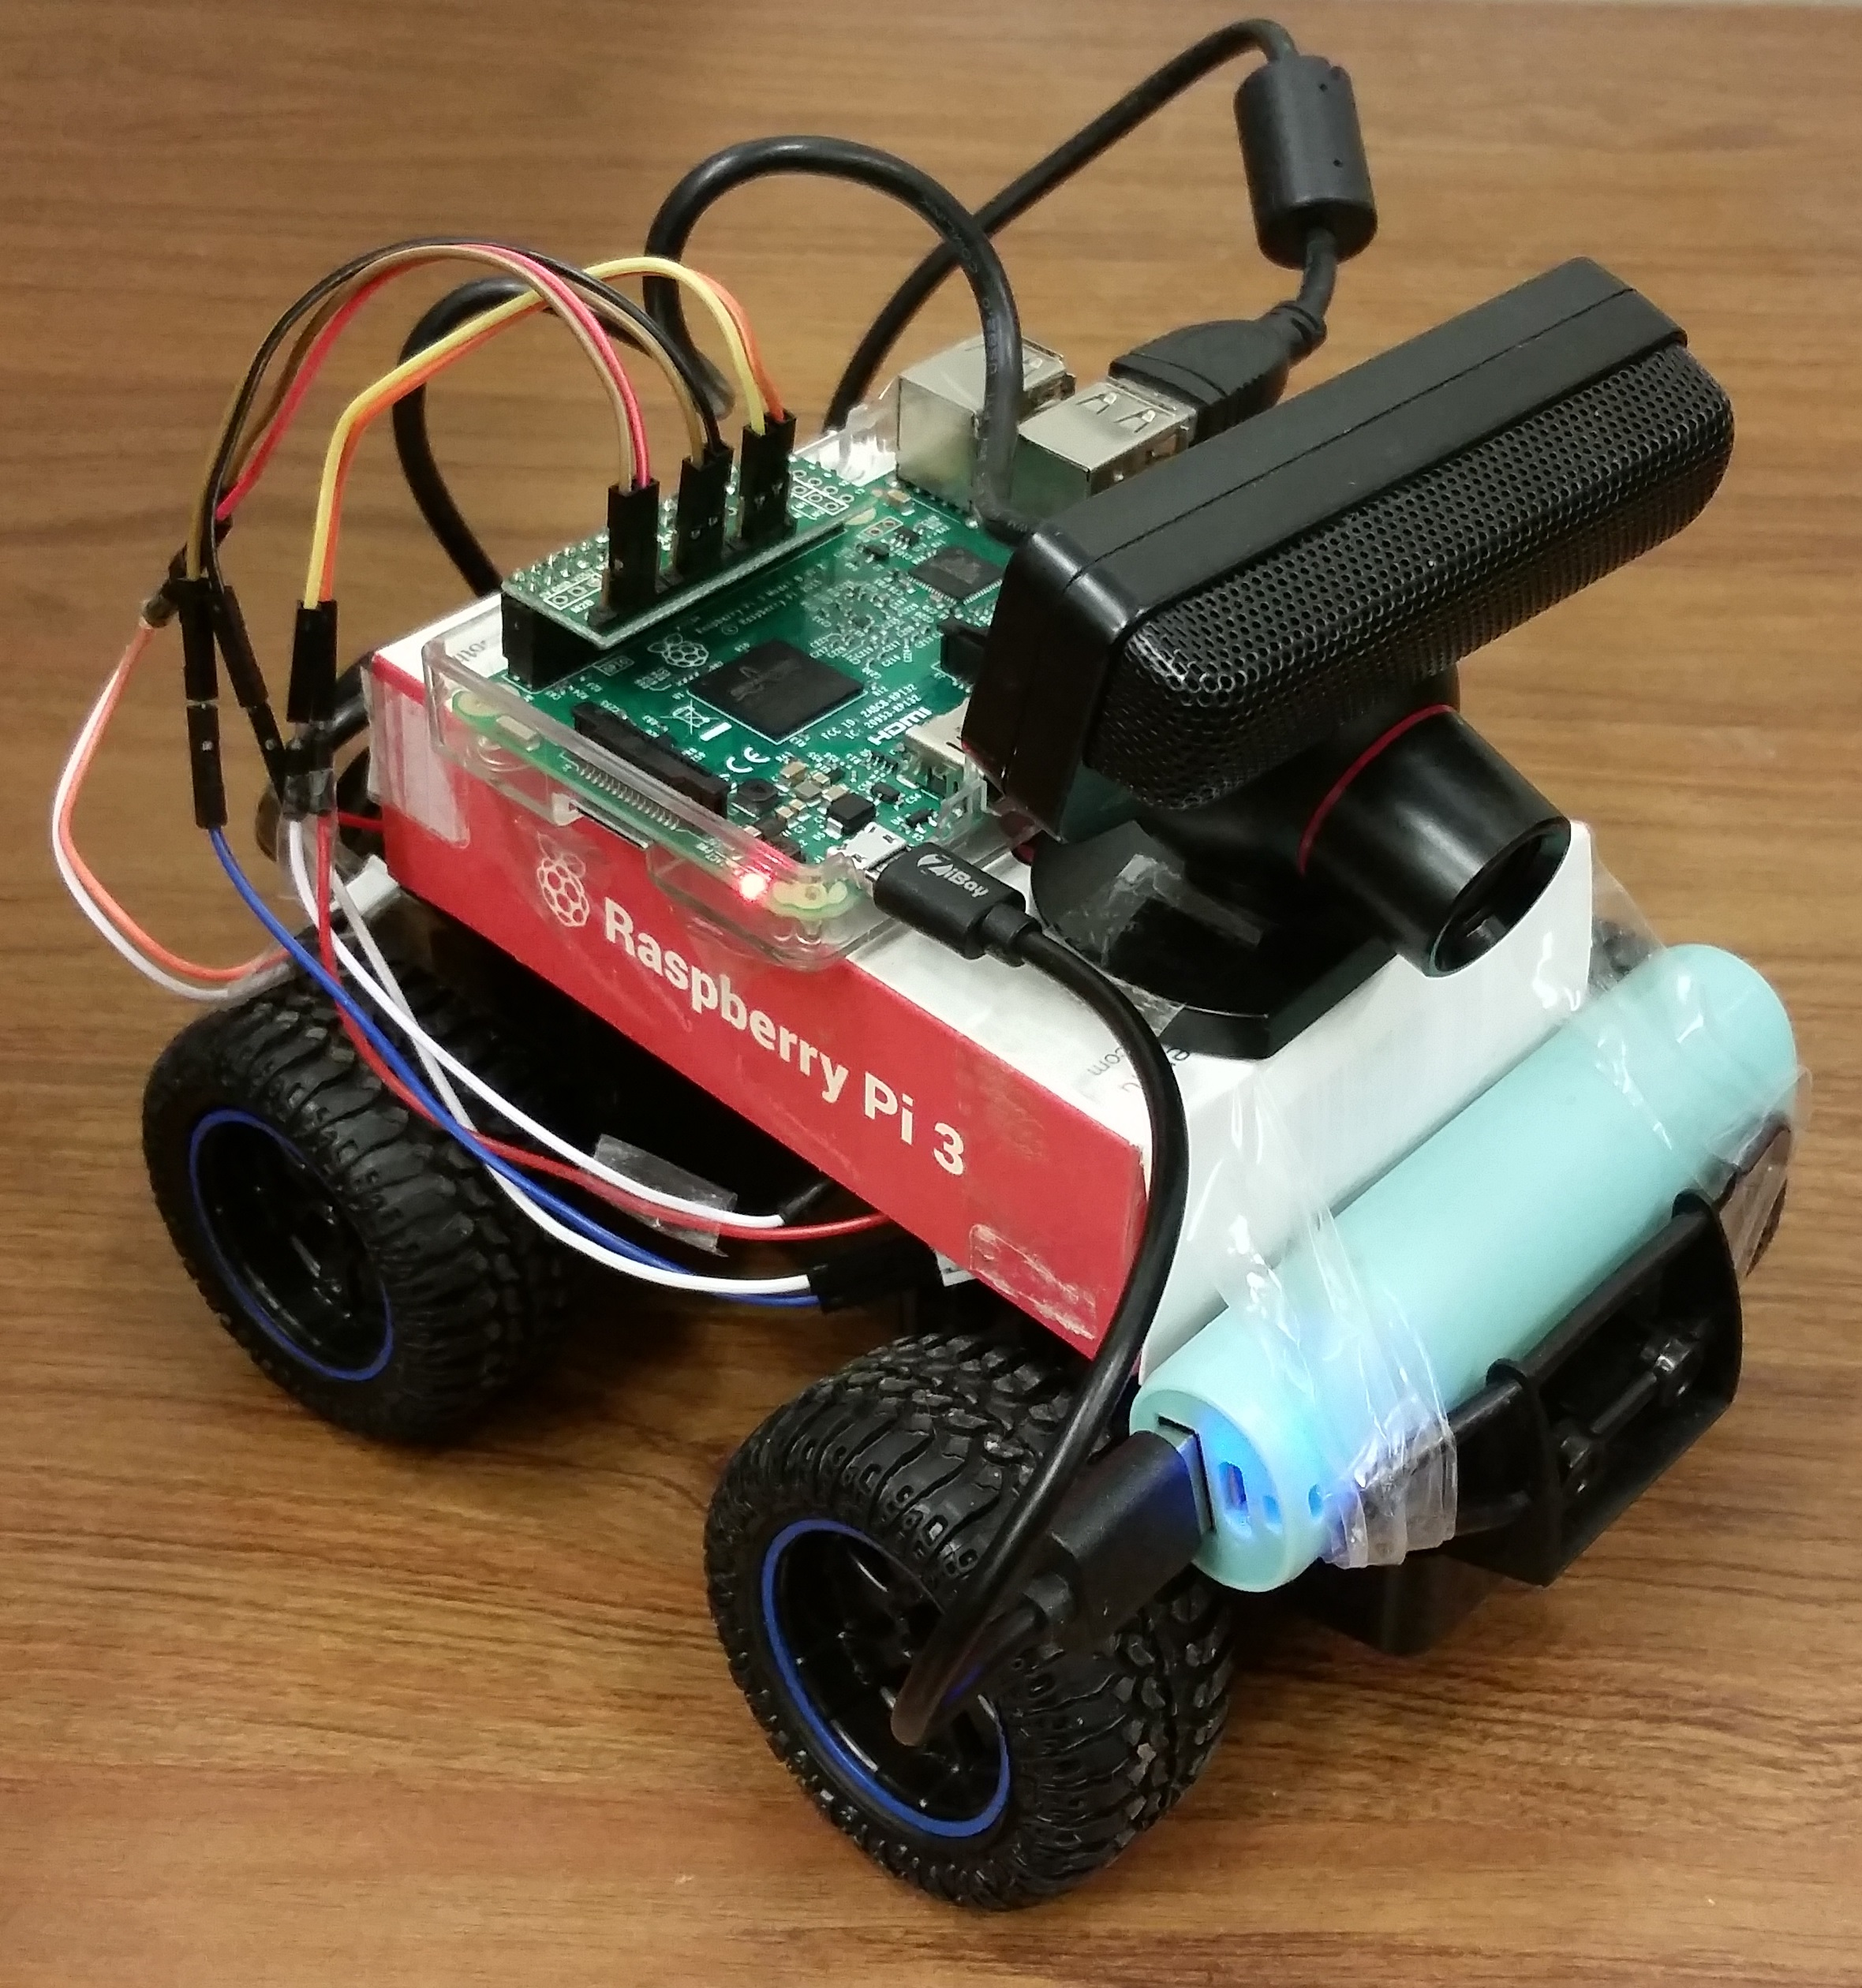
\includegraphics[width=.4\textwidth]{figs/DeepPicar_platform}
  \caption{DeepPicar platform.}
  \label{fig:overview}
\end{figure}

\begin{table}[h]
  \centering
  \begin{tabular}{|c|r|}
    \hline
    Item                    & Cost (\$) \\
    \hline
    Raspberry Pi 3 Model B  & 35 \\
    New Bright 1:24 scale RC car       & 10 \\
    Playstation Eye camera  &  7 \\
    Pololu DRV8835 motor hat&  8 \\
    External battery pack \& misc.   & 10 \\
    \hline
    Total                   & 70 \\
    \hline
  \end{tabular}
  \caption{DeepPicar's bill of materials (BOM)}
  \label{tbl:carbom}
\end{table}

Figure~\ref{fig:overview} shows the DeepPicar, which is comprised of a
set of inexpensive components: a Raspberry Pi 3 Single Board Computer
(SBC), a Pololu DRV8835 motor driver, a Playstation Eye webcam, a
battery, and a 1:24 scale RC car. Table~\ref{tbl:carbom} shows the
estimated cost of the system.

For the neural network architecture, we implement NVIDIA DAVE-2's
convolutional neural network (CNN) using an open-source CNN model in
~\cite{deeptesla}. Note, however, that the CNN model
in~\cite{deeptesla} is considerably larger than NVIDIA's CNN
model as it contains an additional fully-connected layer of
approximately 1.3M additional parameters. We remove the additional
layer to faithfully recreate NVIDIA's original CNN model.
%% The main difference is that we do not utilize a normalization layer, and 
%% instead initialize the weights using a Xavier initialization. 
As in DAVE-2, the CNN takes a raw color image (200x66 RGB pixels)
as input and produces a single steering angle value as output.
Figure~\ref{fig:architecture} shows the network architecture
used in this paper, which is comprised of 9 layers, 250K parameters,
and about 27 million connections as in NVIDIA DAVE-2's architecture.

\begin{figure}[h]
  \centering
  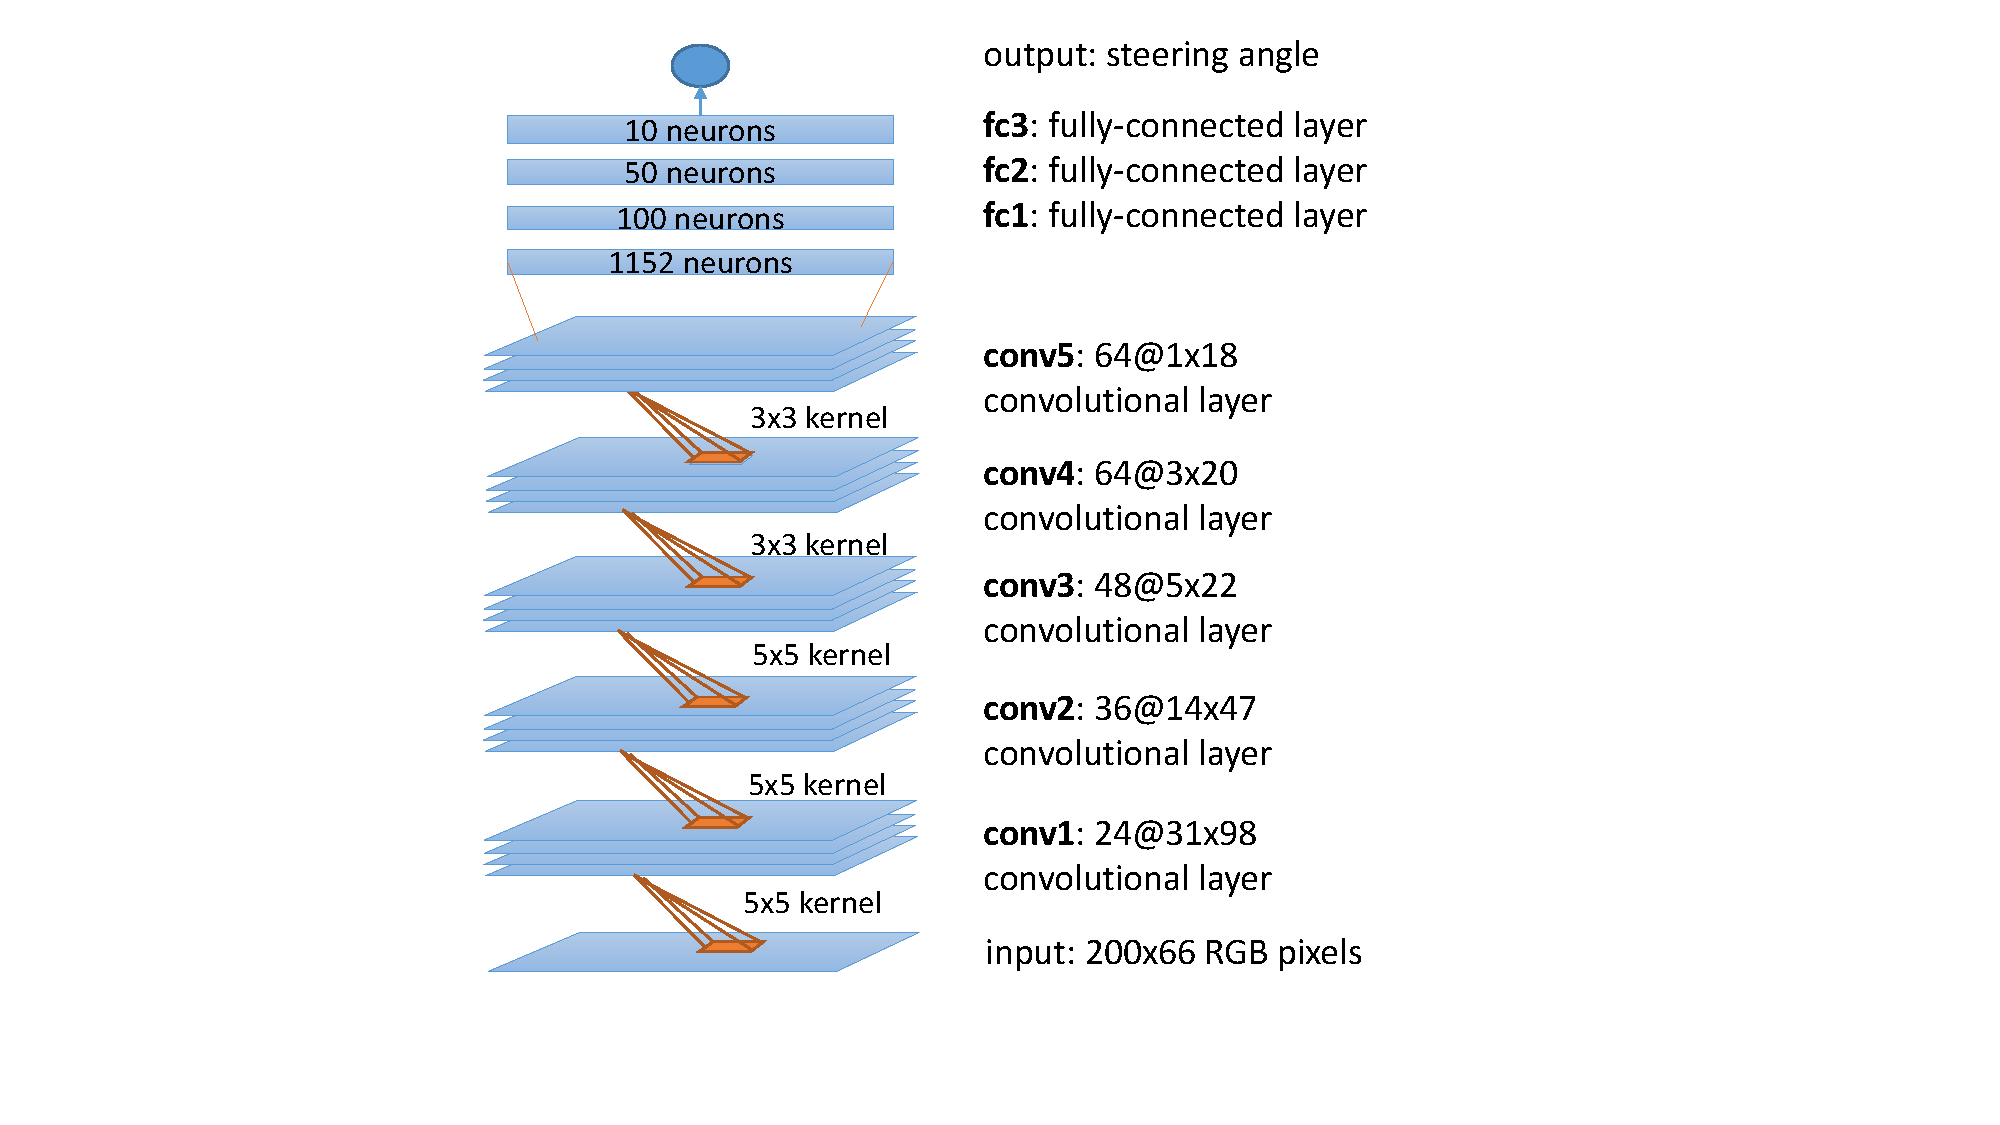
\includegraphics[width=0.4\textwidth]{figs/architecture}
  \caption{DeepPicar's neural network architecture: 9 layers (5
    convolutional, 4 fully-connected layers), 27 million connections,
    250K parameters. The CNN architecture is identical to the one 
	used in NVIDIA's real self-driving car~\cite{Bojarski2016}.}
  \label{fig:architecture}
\end{figure}


%% Note, however,
%% that we did not apply the normalization mentioned
%% in~\cite{Bojarski2016}, as it does not include trainable parameters
%% and its computational demand with respect to the overall CNN
%% processing is minimal.

\begin{figure}[h]
  \centering
  \begin{subfigure}{0.4\textwidth}
    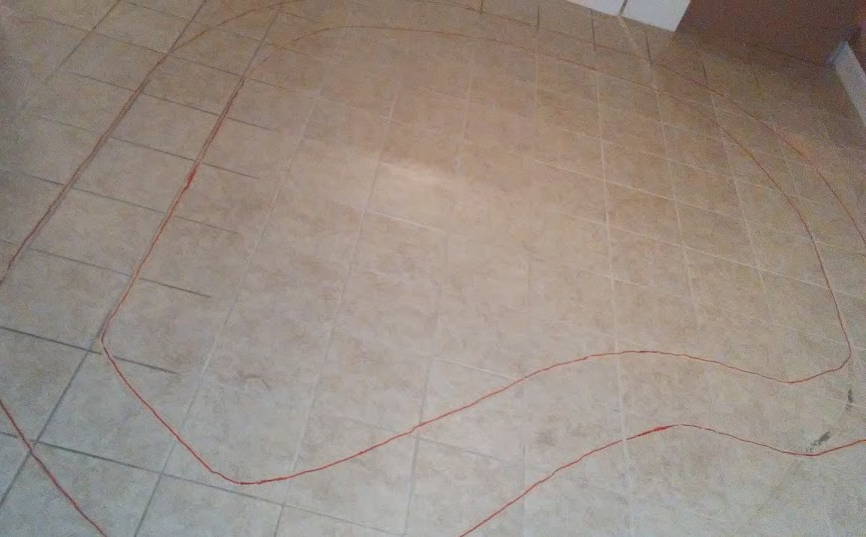
\includegraphics[width=\textwidth]{figs/track-2}
    \caption{Track 1.}
    \label{fig:track}
  \end{subfigure}
  \hfill
  \begin{subfigure}{0.4\textwidth}
    \includegraphics[width=\textwidth]{figs/track-3}
    \caption{Track 2.}
    \label{fig:track2}
  \end{subfigure}
  \caption{Custom tracks used for training/testing}
  \label{fig:tracks}
\end{figure}

% data collection and training.
To collect the training data, a human pilot manually drives the RC car
on tracks we created (Figure~\ref{fig:tracks}) to record
timestamped videos and contol commands. The stored data is then copied 
to a desktop computer, which is equipped with a NVIDIA Titan Xp GPU, 
where we train the network to accelerate training speed.

%% For comparison, training the network on the Raspbeery Pi 3 takes
%% approximately 4 hours, whereas it takes only about 4 minutes on the
%% desktop computer using the Titan Xp GPU.

\begin{figure}[h]
   \lstset{language=python,
           basicstyle=\ttfamily\small,
           keywordstyle=\color{blue}\ttfamily,
           stringstyle=\color{red}\ttfamily,
           commentstyle=\color{green}\ttfamily
          }  
  \lstinputlisting[language=python]{control.py}
  \caption{Control loop}
  \label{fig:controlloop}
\end{figure}

% inferencing on pi3
Once the network is trained on the desktop computer, the trained model
is copied back to the Raspberry Pi 3. The network is then used
by the car's main controlller, which feeds image frames from the web
camera as input to the network in real-time. At each control period,
the network produced steering angle output is converted into the PWM values
of the car's steering motor. Figure~\ref{fig:controlloop} shows simplified 
pseudo code of the controller's main loop. Among the five steps, the 3rd step, 
network inferencing, is the most computationally intensive and dominates the
execution time.

Note that although the steering angle output of the network ($angle$) is
a continuous real value, the RC car platform we used only supports
three discrete angles---left (-30$^{\circ}$), center 
(0$^{\circ}$), and right (+30$^{\circ}$)---as control inputs.
We approximate the network generated real-valued angle to the closest
one of the three angles. Although this may introduce inaccuracy in
control, the observed control performance of the system is respectable,
likely due to the inherently stocastic nature of DNN.

%% In the future, we plan to use a different (more expensive) RC car
%% platform that can precisely control the car's steering angle.

Another factors that can potentially affect the prediction accuracy of
the CNN, are camera and actuator (motor) control latencies. The camera
latency is from the time the camera sensor observes the scene to the
time the computer actually reads the digitized image data. This time
can be noticable depending on the camera used and the data processing
time of the computing platform. Higher camera latency could
negatively affect control performance, because the DNN would analyze
stale scenes. The actuator (motor) control latency from the time
the control output is sent to the steering motor to the time the motor
actually moved at a desired position, which also can takes
considerable time. In our platform, the combined latency is measured
to be around 50 ms, which is reasonble.
%% In other words, %% in the recorded video and control data, 
%% a control action of the CNN appears to be applied 50 ms later.
%% Considering that camera's framerate is 30Hz
%% (33.3 ms/frame), this is about two frames after the control action.
%% We experimentally measured the camera
%% latency and found it to be around 50-100 ms.
If this value is too high, control performance may suffer.
Our initial prototype suffered this problem as the observed latency
was as high as 300 ms, which negatively affected control performance.
For reference, the latency of human perception is known to be as fast
as 13 ms~\cite{ThomasBurger2015}. 
% https://www.pubnub.com/blog/2015-02-09-how-fast-is-realtime-human-perception-and-technology/

Our trained DNN models showed good prediction accuracy, successfully
navigating several different tracks we used for training.
For instance, the DeepPicar could remain on Track 1
(Figure \label{fig:track}) over 10 minutes at a moderate speed (50\%
throttle), at which point we stopped the experiment, and more than one
minute at a higher speed (75\% throttle)~\footnote{Self-driving videos: \url{https://photos.app.goo.gl/q40QFieD5iI9yXU42}
  %% \url{https://photos.app.goo.gl/ce93sU7jPk4ywO8u2}
}. Running at
higher speed is inherently more challenging because the CNN controller
has less time to recover from mistakes (bad predictions).  Also, we
find that the prediction accuracy is significantly affected by the
quality of training data as well as various environmental factors such
as lighting conditions. We plan to investigate more systematic ways
to improve the CNN's prediction accuracies.

We would like to stress, however, that
%% the issues related to the
%% CNN's accuracies have no impact on the \emph{computational 
%% aspects of the system}, and that 
our main focus of this study is not in improving the network accuracy
but in closely replicating the DAVE-2's network architecture and
studying its real-time characteristics, which will be presented in the
subsequent section.


\section{Evaluation}\label{sec:evaluation}

In evaluating the real-time efficacy of the DeepPicar, the methodology is consistent across all 
experiments. The performance of the platform is measured over a set of 1001 video frames that are 
each individually fed to the model. The processing time for the first frame is omitted as, due to 
cache warmup, it is uncharacteristically high and doesn't accurately represent the Picar's capabilities. 
A WCET of 50 ms, or 20 Hz, is used as a baseline to assess the platform's ability to complete all 
necessary real-time operations in a timely manner.

\subsection{Real-Time Operations}
We seek to determine if the DeepPicar is capable of consistently executing all necessary functions 
before their given deadlines. In the case of our platform, it has to process every given frame and get 
the predicted angles from the model within a WCET of 50 ms. In order to determine if this was achievable, 
we tested the platform by running a single model that utilized all 4 cpu cores and measured the time it 
took for each frame to be processed. The performance of the DeepPicar can be seen in Figure 6. We found 
that DeepPicar was able to completely process the vast majority of the provided frames within 50 ms, and 
was unable to do so for very few frames.

\begin{figure}[h]
  \centering
  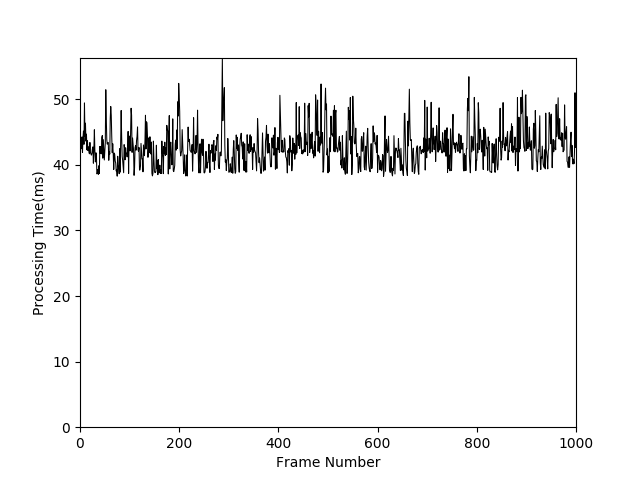
\includegraphics[width=.5\textwidth]{Total_Processing_Time}
  \caption{ Real-time performance of the DeepPicar in processing 1000 frames.}
\end{figure}

In our platform, three main real-time tasks are performed during autonomous operation. In order, these 
operations are: (1) capturing and reading the input frame from the designated camera or video stream, 
(2) preprocessing the acquired frame so that it is compatible with the DNN, and (3) feeding the frame 
to, and getting the angle prediction from, the model. We aim to determine which operation(s), if any, 
require the most time to be performed.

\begin{table}[h]
  \centering
  \begin{tabular} {| l | l | l | l | l |}
    \hline
    \textbf{operation} & \textbf{mean} & \textbf{max} & \textbf{99pct} & \textbf{stdev} \\ \hline 
    Frame Capture & 2.28 & 4.94 & 4.54  & 0.52\\ \hline
    Preprocessing & 3.09 & 4.60 & 3.31 & 0.10 \\ \hline
    Angle Prediction & 37.30 & 51.03 & 45.48 & 2.75 \\  \hline
    Total Time & 42.67 & 56.37 & 50.70 & 2.80 \\
    \hline
  \end{tabular}
  \caption{Real-time performance of DeepPicar for each autonomous vehicle operation performed.}
\end{table}

In order to determine which operation(s) take the longest to execute, we measured the time it 
took for each step to be completed. For this experiment, all four of the Pi's cpu cores were utilized, 
and only one model was run. As is shown in Table II, the angle prediction operation consumes the 
majority of the processing for each frame. Furthermore, the time it takes for the operation to 
complete is volatile, and can range anywhere between 30 ms and 50 ms for any particular frame. On the 
other hand, both the frame capture and preprocessing operations take substantially less time 
and are relatively more consistent in their times, at 2 ms and 3 ms, respectively. 

\subsection{Multicore Performance}
It may not always be the case that all four cores of the Raspberry Pi 3's Cortex A-53 CPU can be used 
solely for the purpose of operating an autonomous vehicle. Thus, we test how the number of cores 
utilized for real-time operations affects the Pi's overall ability to function as an autonomous 
vehicle platform.

\begin{table}[h]
  \centering
  \begin{tabular} {| l | l | l | l | l | l | l | l | l | l |}
    \hline
    \textbf{num cores} & \textbf{mean} & \textbf{max} & \textbf{99pct} & \textbf{stdev} \\ \hline 
    1 & 61.96 & 66.00 & 63.31 & 0.51\\ \hline
    2 & 50.49 & 71.55 & 70.03 & 3.16 \\ \hline
    3 & 48.11 & 72.22 & 58.45 & 4.18 \\ \hline
    4 & 42.67 & 56.37 & 50.70 & 2.80 \\
    \hline
  \end{tabular}
  \caption{Real-time performance of DeepPicar depending on the number of cores used.}
\end{table}

The performance of the DeepPicar is summarized in Table III. The DeepPicar performed better, on average, 
when it utilized more cores. With 4 cores, it was able to meet the vast majority of its deadlines, doing 
so in almost 99\% of the input frames. The platform performed the worst when using only 1 core, 
as it was unable to meet any of its deadlines.  On average, using 3 cores instead of 2 only had a 
performance increase of approximately 2 ms, so the addition of one core in that specific case offers 
relatively little improvement. One important observation is that the performance was more consistent 
when only 1 core was used. As a result, the use of multiple cores is very beneficial in terms of 
reducing the time it takes to complete inference operations, but may result in times that are more 
volatile.

\subsection{Multimodel Performance}
We also test the capability of the DeepPicar to run multiple models at the same time, and whether each 
model can successfully perform within the given deadline. Specifically, the platform is tested in the 
cases of running 2 and 4 models simultaneously. For each case, all models are allocated an equal number 
of cores. That is, 2 models are given 2 cores each and 4 models are given 1 core each.

\begin{figure}[h]
  \centering
  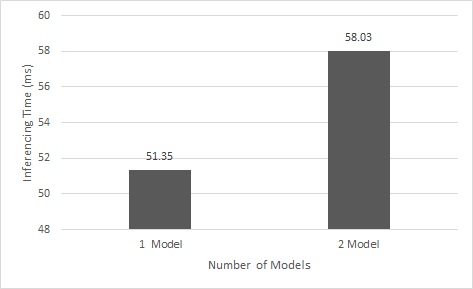
\includegraphics[width=.5\textwidth]{figs/2ModelChart}
  \caption{ Change in inferencing time when 2 models are run concurrently. }
\end{figure}

\begin{table}[h]
\centering
  \begin{tabular} {| l | l | l |}
  \hline
  \textbf{num models} & 1 & 2 \\ \hline
  \textbf{L1 refs} &  3.04E+10 &  3.04E+10 \\ \hline
  \textbf{L1 misses} & 4.78E+08 & 4.91E+08 \\ \hline
  \textbf{L1 miss \%} & 1.58 & 1.61 \\ \hline
  \textbf{L2 refs} & 3.31E+09 &  3.91E+09 \\ \hline
  \textbf{L2 misses} & 3.68E+08 & 4.62E+08 \\ \hline
  \textbf{L2 miss \%} & 11.12 & 10.88 \\ \hline
  \end{tabular}
  \caption{ Effect of 2 simulatneous models on cache accesses. }
\end{table}

The results for the 2 model test are outlined in Figure 3 and Table IV, and the 4 model test is summarized in 
Figure 4 Table V. In the the 2 model test, both of the models showed average inference time increases of around 
5-7 ms, $\sim$10\%, when compared to a baseline of 1 model running on two cores. The difference was even 
greater in the 4 model test, as each model displayed an average inference time increase of 
approximately 15 ms, $\sim$30\%, when compared to a single model running on 1 core.

The increase in inference times, however, was not the result of increased cache misses due to 
additional accesses. For all models, the number of L1 misses was always $\sim$1.6\% of all 
references. In the 2 model test, L2 cache misses remained at $\sim$11\% of all references, and each 
model in the 4 model test missed $\sim$13\% of all L2 references.

\begin{figure}[h]
  \centering
  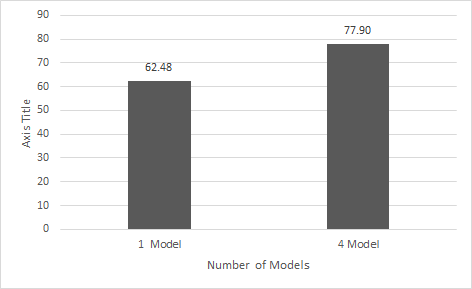
\includegraphics[width=.5\textwidth]{figs/4ModelChart}
  \caption{Change in inferencing time when 4 models are run simultaneously. }
\end{figure}


\begin{table}[h]
\centering
  \begin{tabular} {| l | l | l |}
  \hline
  \textbf{num models} & 1 & 4 \\  \hline
  \textbf{L1 refs} & 2.78E+10 & 2.79E+10 \\ \hline
  \textbf{L1 misses} & 4.36E+08 & 4.53E+08 \\ \hline
  \textbf{L1 miss \%} & 1.57 & 1.63 \\ \hline
  \textbf{L2 refs} & 2.83E+09 & 3.36E+09 \\ \hline 
  \textbf{L2 misses} & 3.59E+08 & 4.43E+08 \\ \hline
  \textbf{L2 miss \%} & 12.68 & 13.19 \\ 
\hline
  \end{tabular}
  \caption{ Effect of 4 concurrent models on cache accesses. }
\end{table}

In all multimodel tests, it was found that a greater number of models run simultaneously resulted in 
interference that led to a noticable increase in the average inferencing time that wasn't 
attributable to a change in cache misses. Instead, the overall time increases can most likely be 
traced to an increase in cache latency. Even if the models had a consistent number of cache hits, it 
is highly probable that the contention for the cache increased the access time for each model, 
consequently increasing the time it took for the models to execute their operations.

In terms of real-time performance under a WCET of 50 ms, the DeepPicar was unsatisfactory in all 
multimodel tests. On average, the 2 model test saw models miss their deadline by 6-8 ms, and the 4 
model test was worse as each model went over their deadlines by 27-29 ms. As a result, it can be 
ascertained that, if a WCET of 50 ms is required, DeepPicar would not be able to perform as necessary.

\subsection{Benchmark Performance}
In order to determine how cache misses affects the performance of the DeepPicar, we test its ability by 
running synthetic benchmarks concurrently with the model. In each experiment, we run a single model on a 
number of cores, and a synthetic benchmark on the remaining idle cores. The effects of the benchmarks can
seen in Figure 9 and Table VI.

\begin{figure}[h]
  \centering
  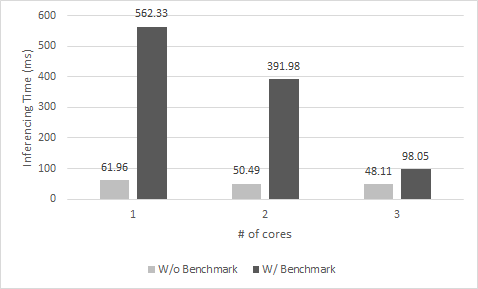
\includegraphics[width=.5\textwidth]{figs/BenchmarkChart}
  \caption{ Effect of benchmarks on inferencing time. }
\end{figure}

\begin{table}[h]
\centering
  \begin{tabular} {| l | l | l | l | l | l |}
  \hline
  \textbf{num cores} & 1 & 2 & 3 \\ \hline
  \textbf{L1 refs} & 3.16E+10 & 3.17E+10 & 3.06E+10 \\ \hline
  \textbf{L1 misses} & 5.41E+08 & 5.35E+08 & 4.98E+08 \\ \hline
  \textbf{L1 miss \%} & 1.71 & 1.69 & 1.62 \\ \hline
  \textbf{L2 refs} & 3.49E+09 & 3.23E+09 & 3.21E+09 \\ \hline
  \textbf{L2 misses} & 8.05E+08 & 7.54E+08 & 4.98E+08 \\ \hline
  \textbf{L2 miss \%} & 23.05 & 23.37 & 15.51 \\ 
  \hline
  \end{tabular}
  \caption{ Effect of benchmarks on cache accesses. }
\end{table}

The presence of the benchmark(s) had a noticable effect on the DeepPicar, with all tests showing 
increases in inferencing operations. The least change happened when the model was run on 3 cores, and a 
single benchmark was run on the final core. Even with a slight increase in the number of L2 cache 
misses, inferencing was able to be completed in under 100 ms. The other tests, however, showed dramatic 
changes when the model was run on 1 and 2 cores. In both instances, L2 misses rise to $\sim$23\% of all 
references. The additional benchmark in the 1 core test was even more detrimental as the average 
inferencing time was at least 150 ms longer than when the model used 2 cores. 

With the introduction of synthetic benchmarks, the DeepPicar failed to comply with the 50 ms WCET across 
all tests run. Even in the best case, inferencing operations take twice as long as the deadline to 
complete. As a result, if benchmarks were required to run during autonomous operation, the DeepPicar 
wouldn't be capable of meeting its deadlines.

\subsection{Summary}
We found that the DeepPicar is capable of successfully completing all necessary inferencing 
operations within a given deadline of 50 ms. Between these operations, it was discovered that the 
angle prediction time of the model was the dominating step in the processing time of a single frame. 
The other operations were found to execute in very little time, with either one taking 5 ms at most.

When running a single model, DeepPicar performed the best when it used all 4 cpu cores, as it was 
able to process a frame in 43 ms on average. This feat can still be accomplished when running a 
single model on 3 cpu cores, and is also possible when using 2 cores. The only time in which the Pi 
can't run a single model under 50 ms is when only 1 core is used. This was also the case when 
multiple models were run concurrently as no models were able to consistently complete inference 
operations in under 50 ms.

However, the DeepPicar was shown to be capable of handling other potential WCETs. If given a larger 
deadline, the capabilities of DeepPicar as an autonomous vehicle platform would be greatly increased. 
For example, if tested with a deadline of 66.67 ms, or 15 fps, the platform would have passed several 
of the experiments performed. In actuality, the DeepPicar would have only been unsatisfactory in the 
4 model test where it would have missed the deadlines by $\sim$10 ms, and the benchmark tests, where 
it would still miss by $\sim$33 ms at best.

\subsection{Performance Requirements}
In the utilization of the Raspberry Pi 3 in our platform, there are a few factors that need to be 
considered and/or enforced in order to guarantee that the Pi is able to consistently perform at a 
desired level. Specifically, these issues all have the potential to negatively affect the cpu clock 
speed/frequency, which would result in decreased performance. While, in the above experiments, the cpu 
operated at a preferred clock speed of 1.2 GHz, it is entirely possible for the cpu to operate at a 
lower frequency if the following problems are not taken into account.

The most notable issue that can affect the cpu clock speed is that of the power supplied to the 
Raspberry Pi. In essence, it is necessary that the Pi be supplied with 2 Amps, as any less could 
hinder the Pi's ability to maintain a 1.2 GHz frequency. In experiments conducted with a power supply that 
only provided 1 Amp, the Pi was unable to sustain a 1.2 GHz clock speed and, instead, fluctuated 
between operating at 600 MHz and 1.2 GHz. As a result, it is necessary, or at least highly 
recommended, that the power supply used for the Raspberry Pi 3 be capable of outputting 2 Amps, 
otherwise optimal performance isn't guaranteed.

Another factor that can affect clock speed is that of the cpu's temperature. Some model operations can 
be computationally intensive, thus it is possible for the temperature of the cpu to become relatively 
high. This can be especially problematic in situations where multiple models are running 
simultaneously on the Pi. Consequently, thermal throttling may be used to decrease the clock 
speed so that the cpu temperature stays at a safe level. Thus the Raspberry Pi may not be suited 
for prolonged use, especially in cases where the workload is relatively larger, such as running multiple 
models. Rather, the Pi seems to be better suited for running in set periods, after which it is turned 
off or made idle so that the cpu is allowed time to cool down.


%
% raspberry p3 spec: https://www.raspberrypi.org/magpi/raspberry-pi-3-specs-benchmarks/

\section{Embedded Computing Platform Comparison}\label{sec:comparison}

In this section, we compare three computing platforms---the Raspberry
Pi 3, the Intel UP~\footnote{http://www.up-board.org/up/} and NVIDIA
Jetson
TX2~\footnote{http://www.nvidia.com/object/embedded-systems-dev-kits-modules.html}---from
the point of view of supporting vision-based end-to-end deep learning
based autonomous vehicles. 
Table~\ref{tbl:platforms} shows architectural features of the three
platforms~\footnote{Note that the GPUs of the Raspberry Pi 3 and Intel
  Up are not used in evaluation due to the lack of software (TensorFlow)
support. Also, the two Denvor cores in Tegra TX2 are not used in
evaluation due to TensorFlow issues.}.
  
Our basic approach is to use the same DeepPicar software, and repeat
the experiments in Section~\ref{sec:evaluation} on each hardware
platform and compare the results. 
For Tegra TX2, we have two different system configurations,
which differ in whether TensorFlow is configured to use its GPU or
only the CPU cores. Thus, the total four system configurations are
compared.

\begin{figure}[h]
  \centering
  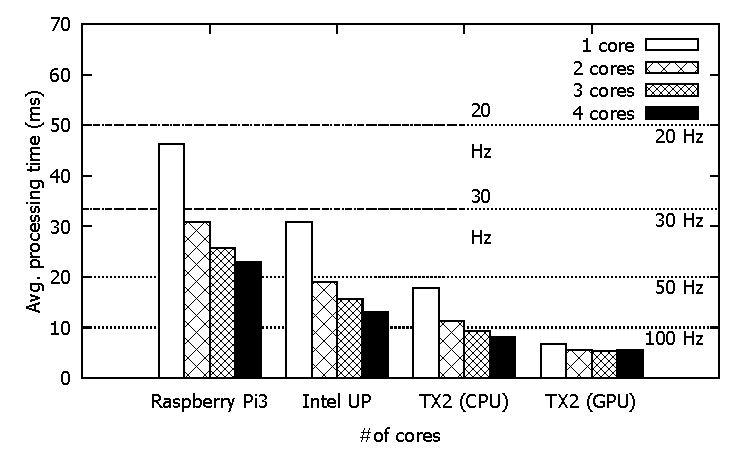
\includegraphics[width=.5\textwidth]{figs/compare_core}
  \caption{Average control loop execution time.} 
  \label{fig:sys_core}
\end{figure}

Figure~\ref{fig:sys_core} shows the average control loop completion
timing of the four system configurations we tested as a function of
the number of CPU cores used.
First, both the Intel UP and Tegra TX2 exhibit superior performance
compared with the Raspberry Pi 3. 
When all four CPU cores are used, the Intel UP is 2.53X faster than
the Pi 3, while TX (CPU) and TX (GPU) are 3.6X and 7.6X times faster,
respectively, than the Pi 3. 
As a result, they are all able to satisfy the 50 ms 
WCET by a clear margin
%%  (in the worst case, the UP Board would 
%% still meet it by $\sim$20 ms) --> where's the data showing this?
, and, in case of TX2, 50 Hz or even 100 Hz real-time control is
feasible with the help of its GPU.


The UP Board and TX2 also performed better in the multimodel tests, 
as is shown in Figure~\ref{fig:sys_model}. Once again, they were able 
to complete control loops in a fraction of the time when compared to 
the Pi. Furthermore, both of the platforms satisfied the 50 ms WCET 
in all experiments, while the Raspberry Pi 3 was unable to do so. As 
such, the UP Board and TX2 display greater potential for the 
simultaneous execution of multiple models during self-driving 
operation, while the Raspberry Pi 3 would struggle to do so.

\begin{figure}[h]
  \centering
  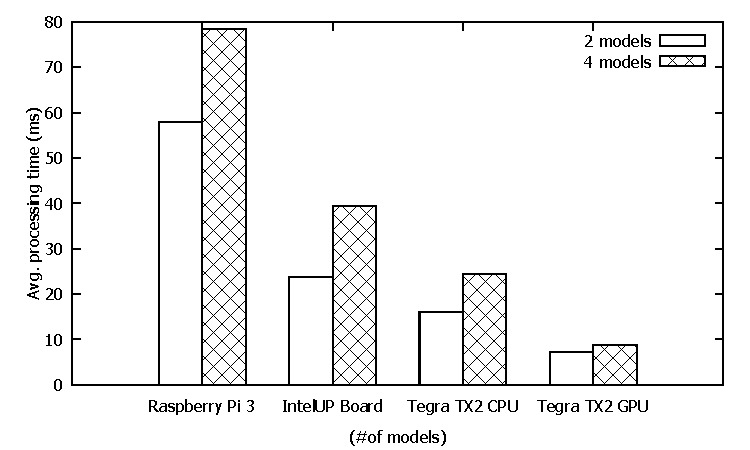
\includegraphics[width=.5\textwidth]{figs/compare_model}
  \caption{Inferencing time across platforms based on number of 
models run concurrently.}
  \label{fig:sys_model}
\end{figure}

Finally, we examined if the performance of the Intel UP Board and 
Tegra TX2 would be affected by the addition of the synthetic 
benchmarks. As summarized in Figure~\ref{fig;sys_bench}, the both 
experienced a change in their inferencing times, but the increases 
were not as drastic as is seen by the Raspberry Pi 3. in the worst 
case, both the UP Board and TX2 (CPU only and GPU) produced times 
that were over two times as large, whereas the Raspberry Pi 3 output 
times that were around 10 times greater. The Intel UP Board was 
successful in completing inferencing operations in under 50 ms when 
benchmarks were run on a maximum of 2 cores, and the TX2 was 
successful in all experiments irrespective of the computing resources 
utilized. Comparetively, both performed better than the Raspberry Pi 
3 which failed to meet its deadlines when any benchmark was 
introduced. As such, it can be concluded that the Intel UP Board 
would be more capable of running computationally heavy processes 
during autonomous driving, and that the Pi wouldn't be able to do the 
same.

\begin{figure}[h]
  \centering
  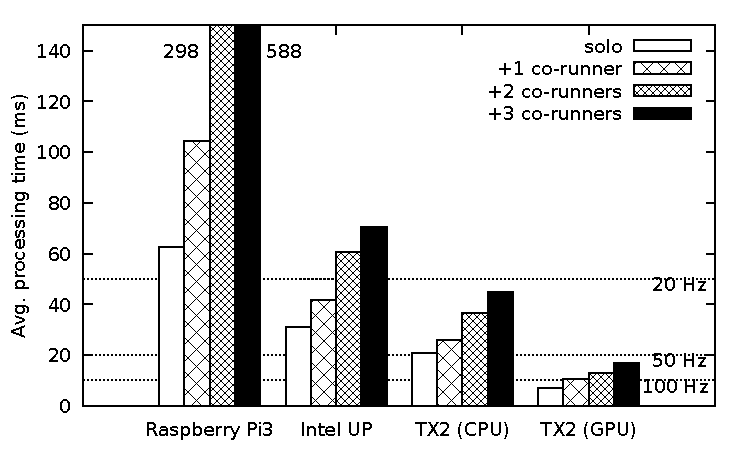
\includegraphics[width=.5\textwidth]{figs/compare_benchmark}
  \caption{Inferencing time across platforms based on number of cores 
used.}
  \label{fig:sys_bench}
\end{figure} 

In the comparison of the real-time capabilities of three embedded 
computing platforms, we found that the Raspberry Pi 3 performed the 
worst. When compared to the Intel UP Board and the NVIDIA Tegra TX2, 
control loops on the Pi were shown to take noticably longer to 
complete, regardless of the number of cores utilized or the number of 
neural network models run simultaneoulsy. The difference was even 
more noticeable in the the addition of computationally heavy 
synthetic benchmarks that had a much more dire effect on the Pi. In 
the worst case, an average control loop on the Pi took an abnormally 
long amount of time to finish. Compared to the TX2 with GPU support, 
those times were 34.8X times greater. From this, we find that the UP 
Board and Tegra TX2 are superior platforms for real-time CNN 
operations. However, due to the Pi's ability to satisfy the 50 ms 
WCET in some experiments, we conclude that the Raspberry Pi 3 is 
feasible for autonomous research.




\section{Related Work}\label{sec:related}

Autonomous vehicles are becoming an increasingly interesting research topic as computing platforms capable of safely processing sensor input into safe vehicle controls become smaller and more affordable.  The model proposed in End-To-End Learning for Self-Driving Cars \cite{Bojarski2016} is viable on a platform as simple as a Raspberry Pi.

Given smaller, affordable platforms with multiple cores and even GPU based parallel processing such as the Tegra X1 \cite{NVIDIA2015} and the recently released Tegra X2 \cite{Amert2017}, allocation and management of available shared CPU and GPU resources \cite{Kim2016} becomes increasingly important.  Research on improving the performance of neural networks \cite{Jouppi2017} also attributes to the viability of using these models in small systems.

Together with hardware and platform improvements, there have been significant improvements in the algorithms such as a neural network algorithm capable of surpassing human level control at atari games \cite{DBLP}.  A popular technique had been to take sensor input and determine a depth map, such as the model used in \cite{Michels:2005}. End-to-end models such as the one used in \cite{Bojarski2016} can improve the efficiency of the model.  Improving the flexibility of the model and it abilty to adapt to different situations and avoiding overfitting to training data continues to be an important topic in autonomous driving \cite{Pomerleau1989}.

Producing large platforms such as DAVE \cite{LeCun:04} has often been the approach to developing the technology for self-driving vehicles.  This approach, while certainly effective, presents a higher barrier to entry for research groups.  Smaller, more focused platforms, such as the one found in \cite{Michels:2005} present a more accesible way forward.

\section{Conclusion}\label{sec:conclusion}
We presented DeepPicar, a low cost autonomous car platform that is
inexpensive to build, but is based on state-of-the-art AI technology:
End-to-end deep learning based real-time control.
Specifically, DeepPicar uses a deep convolutional neural network to
predict steering angles of the car directly from camera input data
in real-time. Importantly, DeepPicar's neural network architecture is
almost identical to that of NVIDIA's real self-driving car. 

Despite the complexity of the neural network, DeepPicar uses a
low-cost Raspberry Pi 3 quad-core computer as its sole computing
resource. We systematically analyzed the real-time characteristics of
the Pi 3 platform in the context of deep-learning based real-time
control applications, with a special emphasis on real-time deep neural
network inferencing.
We also evaluated other, more powerful, embedded computing
platforms to better understand achievable real-time performance of
DeepPicar's deep-learning based control system and the impact of
computing hardware architectures.
We find all tested embedded platforms, including the Pi 3, are capable
of supporting deep-learning based real-time control, from 20 Hz up to
100 Hz, depending on the platform and its system
configuration. However, shared resource contention remains an
important issue that must be considered in applying deep-learning
models on shared memory based embedded computing platforms.

As future work, 
%% we plan to apply shared DRAM resource management
%% techniques~\cite{Yun2013,yun2014rtas} on the DeepPicar platform and
%%evaluate their impact on the real-time performance of the system. 
we plan to improve the prediction accuracy by feeding more data and
upgrading the RC car hardware platform to enable more precise steering
angle control.
%-------------------------------------------------------------------------
\bibliographystyle{abbrv}
\bibliography{reference}

\appendix
\begin{figure*}[t]
  \centering
  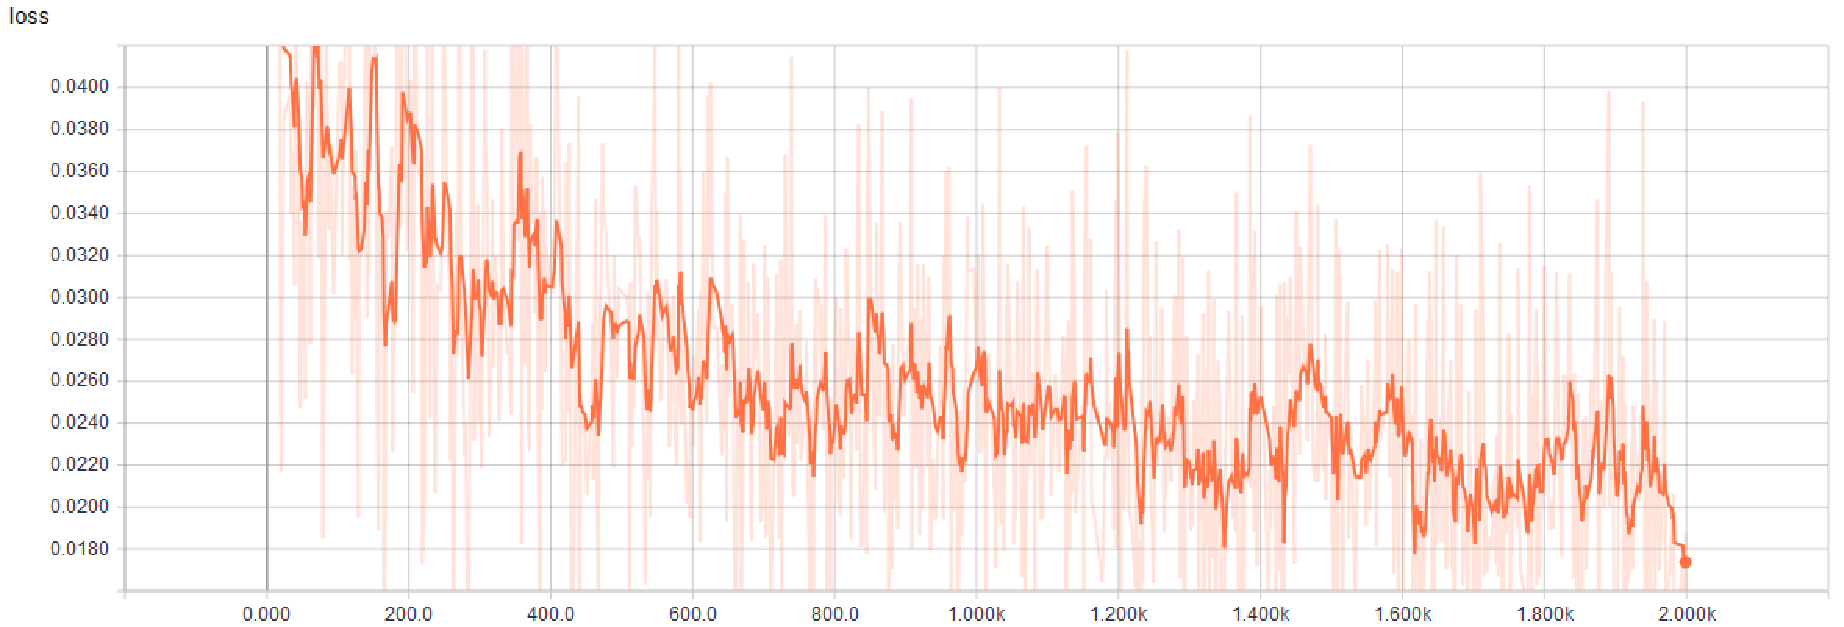
\includegraphics[width=.9\textwidth]{figs/TrainingLoss}
  \caption{Change in loss value throughout training.}
  \label{fig:modelloss}
\end{figure*}


\subsection{DNN Training and Testing}
We have trained and tested the deep neural network with several
different track conditions, different combinations of input
data, and different hyper parameters. In the following paragraphs, we 
describe details on two of the training methods that performed 
reasonably well.

In the first method, we trained the neural network model across a set 
of 30 completed runs on the track seen in Figure~\ref{fig:track} by a
human pilot. Half of the runs saw the car driving one way along the
track, while the remaining half were of the car driving in the
opposite direction on the track.
In total, we collected 2,556 frames for training and 2,609 
frames for validation.
The weights of the network are initialized using a Xavier
initializer~\cite{Glorot2010}, which is known to provide better
initial values than the random weight assignment method.
In each training step, we use a batch
size of 100 frames, which are randomly selected among all the
collected training images, to optimize the network.
We repeat this across 2,000 training steps. When a model was trained
with the  aformentioned data, the training loss was 0.0188 and the
validation  loss was 0.0132.
The change of the loss value over the course of model training can be
seen in Figure~\ref{fig:modelloss}.

In the second method, we use the same data and parameters as  above 
except that now images are labeled as 'curved' and 'straight' and we pick an
equal number of images from each category at each training step to
update the model. In other words, we try to remove bias in selecting
images. We find that the car performed better in practice by applying
this approach as the car displayed a greater ability to stay in the
center of the track (on the white tape).
However, we find that there is a huge discrepency between the training
loss and the validation loss as the former was 0.009, while the latter
was 0.0869---a 10X difference---indicating that the model suffers from
an overfitting problem.

We continue to investigate ways to achieve better prediction accuracy
in training the network, as well as improving the performance of the RC
car platform, especially related to precise steering angle control.

\subsection{System-level Factors Affecting Real-Time Performance}
In using the Raspberry Pi 3 platform, there are a
few system-level factors, namely power supply and temperature, that
need to be considered to achieve consistent and high real-time
performance. 

In all our experiments on the Raspberry Pi 3, the CPU  operated at a
preferred clock speed of 1.2 GHz. However, without care, it is
possible for the CPU to operate at a lower frequency. 

An important factor is CPU thermal throttling, which can affect CPU
clock speed if the CPU temperature is too high (Pi 3's firmware is
configured to throttle at 85C).
DNN model operations are computationally intensive, thus it is
possible for the temperature of the CPU to rise quickly. This can be
especially problematic in situations where multiple DNN models are
running simultaneously on the Pi 3.
If the temperature reaches the threshold, the Pi 3's thermal
throttling kicks in and decreases the clock speed down to 600MHz---
half of the maximum 1.2GHz---so that the CPU's temperature stays at a
safe level.
We found that without proper cooling solutions (heatsink or fan), 
prolonged use of the system would result in CPU frequency decrease
that may affect evaluation.

Another factor to consider is power supply. From our experiences, the
Pi 3 frequency throttling also kicks in when the power source can not
provide the required minimum of 2A current.
In experiments conducted with a power supply that only provided 1 Amp,
the Pi was unable to sustain a 1.2 GHz clock speed, and instead,
fluctuated between operating at 600 MHz and 1.2 GHz. As a result, it
is necessary, or at least highly recommended, that the power supply
used for the Raspberry Pi 3 be capable of outputting 2 Amps, otherwise
optimal performance isn't guaranteed.

Our initial experiment results suffered from these issues, after which
we always carefully monitored the current operating frequencies of the
CPU cores during the experiments to ensure the correctness and
repeatability of the results.

\end{document}
